\documentclass[dvipsnames,presentation,aspectratio=169,14pt]{beamer}
\usepackage{hastingstheme}
\usepackage{qrcode}
\titlegraphic{
\includegraphics[scale=.35]{static_figures/du_bn.pdf}}
\author{\large Massimiliano Fasi}
\date{}

\usepackage{pgfplots}

% \usepackage{template}
% \renewcommand{\authorname}{Lawrence Mitchell\inst{*}}
\renewcommand{\authoremail}{\inst{*}\texttt{lawrence.mitchell@durham.ac.uk}}

% \renewcommand{\sessionnumber}{1}
% \renewcommand{\sessiontitle}{Introduction \& Overview}

\begin{document}

\title{\firasemibold\color{White}%
  {\fontsize{20}{0}\selectfont SESSION 1\\
    \fontsize{40}{40}\selectfont Overview\par}}
\titleslide

\section{Introduction}

\begin{frame}
  \frametitle{One-slide course summary}

  \begin{challenge}{Fundamental question}
    I would like this code to run faster: how do I know \structure{what} to do?
  \end{challenge}
  \pause
  \begin{answer}{Performance models \& measurements}
    We can treat the computer as an experimental system:
    \begin{enumerate}
    \item Measure performance

    \item Construct \emph{models} that explain performance

    \item Apply appropriate optimisations
    \end{enumerate}
  \end{answer}
\end{frame}

\begin{frame}
  \frametitle{Course overview}
  \begin{columns}
    \begin{column}{0.6\linewidth}
      \begin{itemize}[itemsep=5pt]
      \item Computer architecture overview
      \item Basics of performance engineering
      \item Tools: CPU topology and \emph{affinity}
      \item Roofline performance model
      \item Tools: Performance counters
      \item \textcolor{gray}{Vectorisation (SIMD programming)}
      \item Data layout transformations
      \end{itemize}
    \end{column}
    \hfill
    \begin{column}{0.3\linewidth}
      \centering
      {\color{palette2}%
        \qrcode[height=1.6in]{https://scicomp-durham.github.io/COMP52315/}
      }
      \newline
    \end{column}
  \end{columns}
  \centering
  \vskip 20pt

  \url{https://scicomp-durham.github.io/COMP52315/}
\end{frame}

\begin{frame}
  \frametitle{What you will need}
  \begin{itemize}[itemsep=5pt]
  \item Hamilton account (which you should already have)
  \item familiarity with basic shell commands
  \item \texttt{likwid} tools, already available on Hamilton
  \end{itemize}
  \vskip 15pt
  \begin{challenge}{Code?}
    This course is about \structure{running} code, not writing it.
  \end{challenge}
\end{frame}

\section{Resources in stored-program computers}

\begin{frame}
  \frametitle{Stored-program architecture}
  \begin{center}
    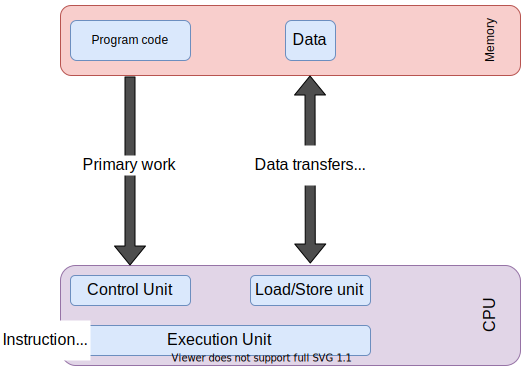
\includegraphics[height=0.8\textheight]{figures/CPU.png}
  \end{center}
\end{frame}

\begin{frame}
  \frametitle{Resource bottlenecks: instruction execution}
  \begin{itemize}[itemsep=5pt]
  \item Primary resource of the processor.
  \item Measure is instruction throughput (instructions/second).
  \item First HW design goal is to \emph{increase} instruction throughput.
  \end{itemize}
  \centering
  \vskip 5pt
  Performance depends on how fast the CPU \structure{retires} instructions.
  \vskip 5pt
  \pause
  \begin{block}{Retired instruction}
    \begin{itemize}[itemsep=5pt]
    \item CPUs execute more instructions than needed by program flow.
    \item ``Retired instruction'' are those whose results are \structure{stored}.
    \end{itemize}
  \end{block}
\end{frame}

\begin{frame}[fragile]
  \frametitle{Example: adding two arrays}\small
\begin{minted}{c}
               for (int i = 0; i < N; i++)
                   a[i] = a[i] + b[i];
\end{minted}
  \vskip 11pt
  \pause
  \hrule
  \vskip 18pt
  \centering
  \begin{columns}[t]
    \hfill
    \begin{column}{0.4\textwidth}
      \structure{User view}\\[4pt]

      Work is $N$ flops (additions)
    \end{column}
    \hfill
    \begin{column}{0.4\textwidth}
      \structure{Processor view}\\[4pt]

      Work is 6$N$ instructions
\begin{minted}{c}
.top
LOAD r1 = a[i]
LOAD r2 = b[i]
ADD  r1 = r1 + r2
STORE a[i] = r1
INCREMENT i
GOTO .top IF i < N
\end{minted}
    \end{column}
  \end{columns}
\end{frame}

\begin{frame}
  \frametitle{Mismatch}

  \centering
  \begin{columns}[t]
    \begin{column}{0.4\textwidth}
      \structure{User view}\\[4pt]

      Work is $N$ flops (additions)
    \end{column}
    \begin{column}{0.4\textwidth}
      \structure{Processor view}\\[4pt]

      Work is $6N$ instructions
    \end{column}
  \end{columns}

  \vskip 20pt

  \begin{challenge}{Mismatch}
    \begin{itemize}[itemsep = 5pt]
    \item Processor designers: all instructions are ``work''.
    \item Code developers: instructions I write are ``work''.
    \end{itemize}
  \end{challenge}
\end{frame}

\begin{frame}
  \frametitle{Hardware for programmers}
  \begin{center}
    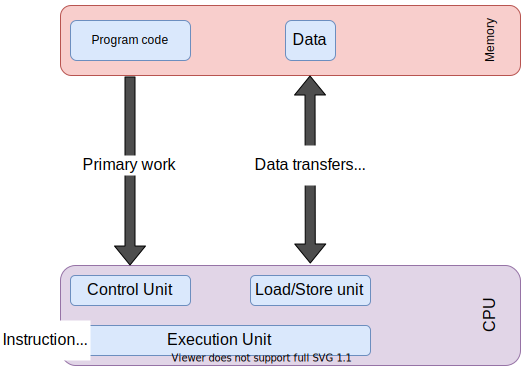
\includegraphics[height=0.8\textheight]{figures/CPU.png}
  \end{center}
\end{frame}

\begin{frame}[fragile]
  \frametitle{Resource bottlenecks: data transfer}
  \begin{itemize}[itemsep=8pt]
  \item From memory to CPU and back.
  \item Consequence of instruction execution.
  \item Secondary resource.
  \item Measure is bandwidth (bytes/second).
  \item Bandwidth determined by load/store rate and HW limits.
  \end{itemize}

\end{frame}

\begin{frame}[fragile]
  \frametitle{Example: adding two arrays}
\begin{minted}{c}
            for (int i = 0; i < N; i++)
                a[i] = a[i] + b[i];
\end{minted}

  \vskip 11pt
  Data transfers (double precision floats):
  \vskip 15pt

\begin{minted}{c}
            LOAD  r1 = a[i] /* 8 bytes */
            LOAD  r2 = b[i] /* 8 bytes */
            STORE a[i] = r1 /* 8 bytes */
\end{minted}

  \vskip 15pt

  24 bytes of data movement per loop iteration.
  % \end{exampleblock}
\end{frame}

\begin{frame}
  \frametitle{Understanding the performance of some code}

  \begin{challenge}{Core question}
    \begin{center}
      \structure{What is the resource bottleneck?}
    \end{center}
    \begin{itemize}[itemsep=5pt]
    \item Instruction execution?
    \item Data transfer?
    \end{itemize}
  \end{challenge}
  \pause
  \begin{answer}{Tools to find an answer}
    \begin{itemize}[itemsep=5pt]
    \item Measurements
    \item Models
    \end{itemize}
  \end{answer}
\end{frame}

\colorlet{cpufg}{Blue}
\colorlet{cpubg}{Blue!15}
\colorlet{memfg}{BrickRed}
\colorlet{membg}{BrickRed!15}
\colorlet{incol}{Purple}
\colorlet{outcol}{Cyan}
\colorlet{recfg}{PineGreen}
\colorlet{recbg}{PineGreen!15}
\colorlet{buscol}{Gray}

\newcommand{\drawblocks}[4]{%
  % Bus
  \draw[<->,draw=buscol] (2.5,0) -- (2.5,-1);

  % Control
  \draw[rounded corners,draw=cpufg,fill=cpubg]
  (0,0) rectangle (5,1.5);
  \draw[rounded corners,draw=cpufg,text=cpufg,fill=cpubg]
  (0.25,0.25) rectangle (1.25,1.25) node[midway] {#1};
  \draw[rounded corners,draw=cpufg,text=cpufg,fill=cpubg]
  (1.5,0.25) rectangle (4.75,1.25) node[midway] {#2};

  % I/O
  \draw[<-,draw=incol,text=incol]
  (5,-1.5) -- (7,-1.5) node[midway, above] {I};
  \draw[->,draw=outcol,text=outcol]
  (5,-2.0) -- (7,-2.0) node[midway, below] {O};

  % Memory
  \draw[rounded corners,draw=memfg,text=memfg,fill=membg]
  (0,-1) rectangle (5,-2.5);
  \node[text=memfg] at (0.75,-1.75) {#3};
  \node[text=memfg,anchor=west] at (2.,-1.5)
  {\firamedium\footnotesize INSTRUCTIONS};
  \node[text=memfg,anchor=west] at (2.,-2.0)
  {\firamedium\footnotesize DATA};
  % \draw[rounded corners,draw=memfg,text=memfg,fill=membg]
  % (0.25,-1.5) rectangle (2.25,-2.25) node[midway] {\footnotesize INSTRUCTIONS};
  % \draw[rounded corners,draw=memfg,text=memfg,fill=membg]
  % (0,-) rectangle (5,-2.5) node[midway] {\footnotesize DATA};

  % Recording medium
  \draw[rounded corners,draw=recfg,text=recfg,fill=recbg,dashed]
  (7,-2.5) rectangle (8.5,1.5) node[midway] {#4};
}

\begin{frame}
  \frametitle{The ``Princeton'' architecture}

  \vfill

  \begin{columns}
    \begin{column}[c]{0.5\textwidth}
      \centering
      \begin{tikzpicture}[ultra thick, scale=1]
        \drawblocks{CC}{CA}{M}{R}
      \end{tikzpicture}
    \end{column}
    \qquad
    \begin{column}[c]{0.35\textwidth}
      \setlength\tabcolsep{5pt}
      \begin{tabular}{ll}
        \color{cpufg}CC  & \color{cpufg}central control\\
        \color{cpufg}CA  & \color{cpufg}central arithmetic\\
        \color{memfg}M   & \color{memfg}memory\\
        \color{incol}I   & \color{incol}input\\
        \color{outcol}O  & \color{outcol}output\\
        \color{recfg}R   & \color{recfg}recording medium
      \end{tabular}
    \end{column}
  \end{columns}

  \vfill

  \begin{thebibliography}{99}
  \bibitem{item1} \mybibitem{John~von~Neumann}
    {http://dx.doi.org/10.1109/85.238389}
    {First draft of a report on the EDVAC}
    {Incomplete report}
    {1--101}{30 June 1945}{100}
  \end{thebibliography}
\end{frame}

\begin{frame}
  \frametitle{The ``Princeton architecture''}
  % \begin{columns}
  %   \begin{column}{0.5\textwidth}
  \begin{itemize}
  \item Used by programming languages
  \item Sequential model
  \item In-order execution
  \item Simple
  \item<2> Realistic
    for 1945
  \end{itemize}
  % \end{itemize}
  % \end{column}
  % \begin{column}{0.5\textwidth}
  %   \begin{center}
  %     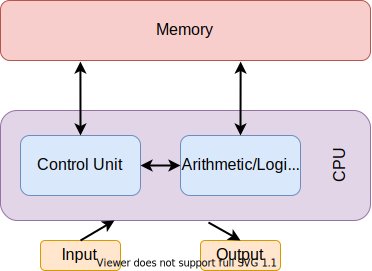
\includegraphics[height=0.6\textheight]{figures/vonneumann.png}
  %   \end{center}
  % \end{column}
  % \end{columns}
  \vfill
  \pause

  \begin{thebibliography}{99}
  \bibitem{item1} \mybibitem{John~von~Neumann}
    {http://dx.doi.org/10.1109/85.238389}
    {First draft of a report on the EDVAC}
    {Incomplete report}
    {1--101}{30 June 1945}{100}
  \end{thebibliography}
\end{frame}

\transslide{\large What has changed in the last 77 years?}





\begin{frame}
  \frametitle{The ``Princeton'' architecture today}

  \begin{columns}
    \begin{column}[c]{0.5\textwidth}
      \centering
      \begin{tikzpicture}[ultra thick, scale=1]
        \drawblocks
        {\only<1>{CC}\only<2->{CU}}
        {\only<1>{CA}\only<2->{ALU}}
        {\only<1>{M}\only<2->{RAM}}
        {\only<1>{R}\only<2->{}}

        % CPU
        \node [anchor=south west,text=cpufg] at (0,1.5)
        {\only<1>{\phantom{CPU}}\only<2->{CPU}};
        % Bus
        \node [anchor=west,text=buscol] at (2.5,-0.5) {\only<2->{BUS}};
      \end{tikzpicture}
    \end{column}
    \qquad
    \begin{column}[c]{0.35\textwidth}
      \setlength\tabcolsep{5pt}
      \onslide<1>{%
        \begin{tabular}{ll}
          &\\
          \color{cpufg}CC & \color{cpufg}central control\\
          \color{cpufg}CA & \color{cpufg}central arithmetic\\
          \color{memfg}M  & \color{memfg}memory\\
          \color{incol}I  & \color{incol}input\\
          \color{outcol}O  & \color{outcol}output\\
          \color{recfg}R  & \color{recfg}recording medium
        \end{tabular}}%
    \end{column}
  \end{columns}

  \vspace{20pt}

  \onslide<3>{%
    \structure{THE ONE FEATURE:} both instructions and data reside in
    memory.\\[5pt]
  \hfill But CPUs are \structure{much} more complicated today!}
\end{frame}

\begin{frame}
  \frametitle{On-chip memory}
  \hspace{6pt}
  \begin{tikzpicture}[ultra thick]
    % Control
    \node[anchor=south west,text=cpufg] at (0,1.5) {CPU};

    \draw[rounded corners,draw=cpufg,fill=cpubg] (0,-4) rectangle (13,1.5);

    \draw[rounded corners,draw=cpufg,text=cpufg,fill=cpubg]
    (0.25,0.25) rectangle (1.25,1.25) node[midway] {CU};

    \draw[rounded corners,draw=cpufg,text=cpufg,fill=cpubg]
    (1.5,0.25) rectangle (4.75,1.25) node[midway] {ALU};

    \draw[rounded corners,draw=cpufg,fill=cpubg,text=cpufg]
    (0.25,-3.75) rectangle (4.75,-0)
    node[midway,above=0.30] (M) {REGISTERS}
    node [below of=M,text width=6cm,align=center]
    {\small \mbox{current instructions} current data};

    \draw[rounded corners,draw=cpufg,fill=cpubg,text=cpufg]
    (5,-3.75) rectangle (12.75,1.25)
    node[midway,above=0.25] (MC) {CACHE MEMORY}
    node [below of=MC,text width=6cm,align=center]
    {\small \mbox{past/future instructions} past/future data};
  \end{tikzpicture}
\end{frame}

\begin{frame}
  \frametitle{Definitions}
  \begin{tabular}{ll}
    \structure{Cycle} & unit of execution of CPU\\[11pt]
    \structure{Frequency} & \# cycles per second (measured in Hz)\\[11pt]
    \structure{Latency} & \# cycles to execute given instruction\\[11pt]
    \structure{Throughput} & \# instructions that can run simultaneously\\[11pt]
  \end{tabular}
\end{frame}

\newcommand{\myanswer}[1]{{\vspace{3pt}\color{MidnightBlue}\textit{#1}}}

\begin{frame}[fragile]
  \frametitle{Problem}
  Most instructions have a \emph{latency} of \emph{more than one} clock cycle.
  \vskip 11pt
  \begin{columns}
    \begin{column}{0.4\textwidth}
\begin{minted}{c}
 LOAD r1 = a[i]
 LOAD r2 = b[i]
 ADD  r1 = r1 + r2
 STORE a[i] = r1
 INCREMENT i
\end{minted}
    \end{column}
    \begin{column}{0.6\textwidth}
      What happens if:\\[7pt]
      \begin{itemize}[itemsep=7pt]
      \item all instruction have latency 1?

        \myanswer{No ``wasted'' cycles.}

      \item \texttt{ADD} has latency 3?

        \myanswer{Two ``wasted'' cycles before \texttt{STORE}.}
      \end{itemize}
    \end{column}
  \end{columns}
\end{frame}

\begin{frame}
  \frametitle{In pictures}
  \begin{center}
    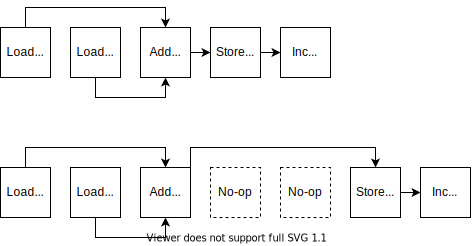
\includegraphics[width=0.9\textwidth]{figures/addlatency.png}
  \end{center}
\end{frame}

\begin{frame}
  \frametitle{Strategies for faster chips}
  \begin{enumerate}[itemsep=8pt]
  \item Increase clock speed (more cycles per second)
  \item Parallelism
    \begin{itemize}[itemsep=5pt]
    \item data-level parallelism
    \item instruction-level parallelism
    \end{itemize}
  \item Specialisation (optimised hardware units)
  \end{enumerate}
\end{frame}

\begin{frame}
  \frametitle{Increasing clock speed}
  \begin{center}
    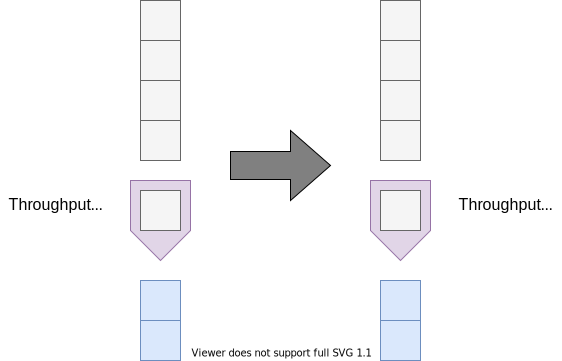
\includegraphics[height=0.8\textheight]{figures/clockincrease.png}
  \end{center}
\end{frame}

\begin{frame}
  \frametitle{Increasing clock speed}
    \begin{answer}{Easy for the programmer}
      Architecture is unchanged, everything just happens faster!
    \end{answer}
    \begin{challenge}{Limitations}
      \begin{itemize}[itemsep=5pt]
      \item Limited by physical impossibility to cool chip.
      \item Clock speeds have been approximately constant for 10 years.
      \end{itemize}
    \end{challenge}
\end{frame}

\begin{frame}
  \frametitle{Increasing parallelism}
  \begin{center}
    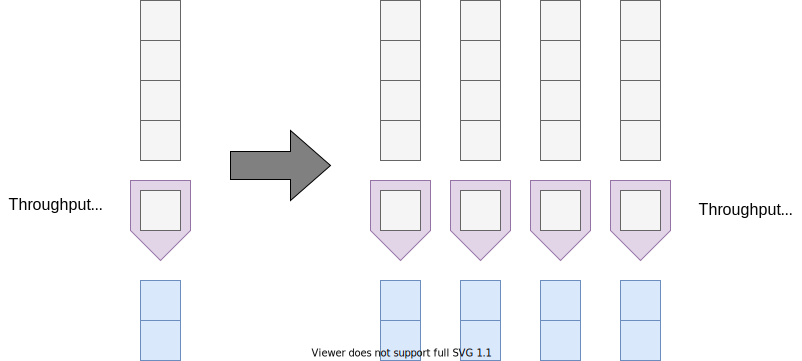
\includegraphics[height=0.8\textheight]{figures/parallelismincrease.png}
  \end{center}
\end{frame}

\begin{frame}
  \frametitle{Increasing parallelism}
  \begin{challenge}{Problems}
    \begin{itemize}[itemsep=7pt]
    \item Need enough parallel work

    \item No dependencies between work

    \item Mostly pushes problem onto programmer
    \end{itemize}
  \end{challenge}
\end{frame}

\begin{frame}
  \frametitle{Instruction-level parallelism: pipelining}
  \vskip -20pt
  \begin{columns}
    \begin{column}{0.33\textwidth}\small
      Split each instruction into
      \begin{itemize}
      \item fetch
      \item decode
      \item execute
      \item write
      \end{itemize}
and use a pipeline.
    \end{column}
    \begin{column}{0.6\textwidth}
      \begin{center}
        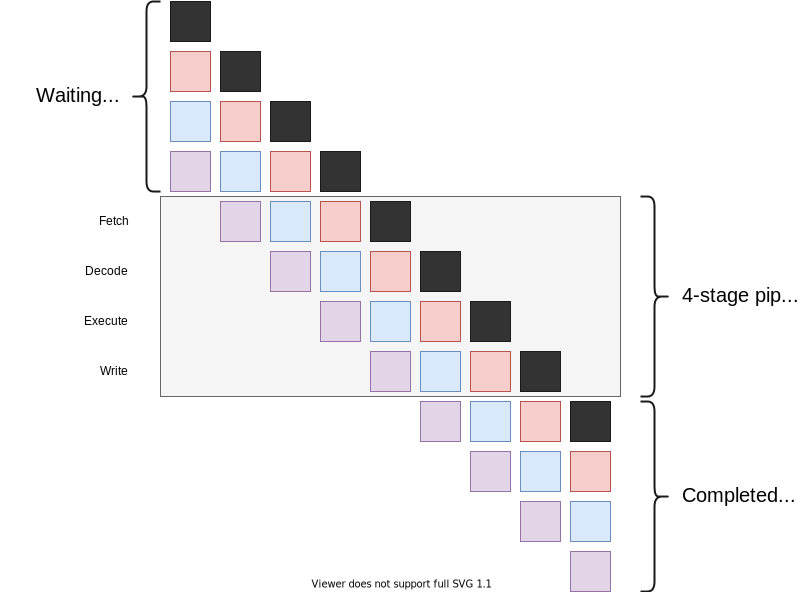
\includegraphics[height=0.85\textheight]{figures/pipeline.png}
      \end{center}
    \end{column}
  \end{columns}
\end{frame}

\begin{frame}
  \frametitle{Instruction-level parallelism: superscalar}
  \begin{center}
    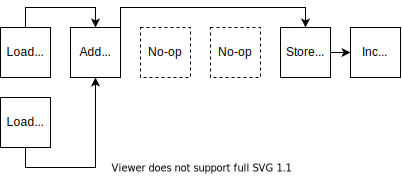
\includegraphics[width=0.9\textwidth]{figures/addsuperscalar.png}
  \end{center}
  Instructions with no dependencies can be issued \structure{simultaneously}.
\end{frame}

\begin{frame}
  \frametitle{Instruction-level parallelism: out-of-order}
  Instruction ordering is based on availability of
  \vskip 5pt
  \begin{itemize}[itemsep=6pt]
  \item input data
  \item execution units
  \end{itemize}
  \vskip 5pt
  rather than order in the program.
  \hfill
  \begin{center}
    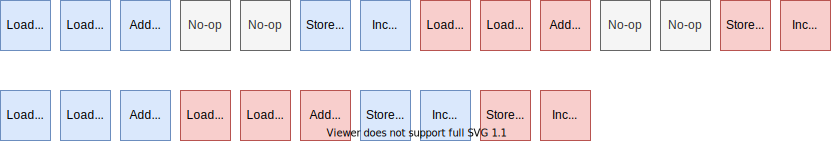
\includegraphics[width=\textwidth]{figures/addoutoforder.png}
  \end{center}
\end{frame}

\begin{frame}[fragile]
  \frametitle{Data parallelism: SIMD vectorisation}

  \begin{exampleblock}{Summing arrays again}
\begin{minted}{c}
double *a, *b, *c;
...
for (size_t i = 0; i < N; i++)
  c[i] = a[i] + b[i];
\end{minted}

    \vskip 5pt

    Instruction throughput can be a bottleneck here.

    \vskip 3pt

    \structure{Vectorisation:} make instructions operate on more data at once.

    \vskip 3pt
  \end{exampleblock}

  \vskip 8pt

  Vectorisation is critical for \structure{single-core} performance.

\end{frame}

\begin{frame}[fragile]
  \frametitle{SIMD execution}
  \vskip -10pt

  \begin{columns}[c]
    \begin{column}{0.5\textwidth}
\begin{minted}{c}
double *a, *b, *c;
...
for (i = 0; i < N; i++)
  c[i] = a[i] + b[i];
\end{minted}

      \vspace{\baselineskip}
      Register widths:\\[6pt]

      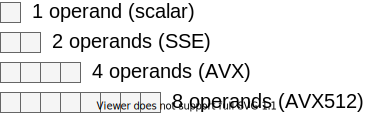
\includegraphics[width=\textwidth]{figures/registerwidth.png}
    \end{column}
    \begin{column}{0.5\textwidth}
      \only<1>{%
        \begin{center}
          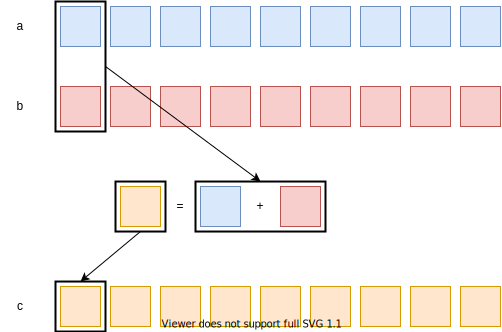
\includegraphics[width=0.7\textwidth]{figures/scalaradd.png}

          \vskip 5pt
          Scalar addition
        \end{center}}%
      \only<2>{%
        \begin{center}
          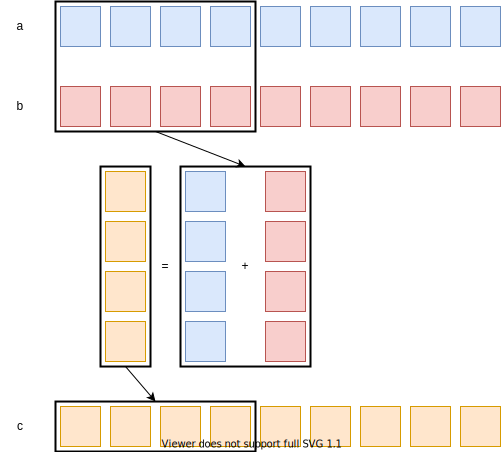
\includegraphics[width=0.7\textwidth]{figures/vectoradd.png}

          \vskip 5pt
          AVX addition
        \end{center}}
    \end{column}
  \end{columns}
\end{frame}

\section{Example and exercise}

\begin{frame}[fragile]
  \frametitle{Example: sum reduction}

  How fast can this code run if all data are in L1 cache?

  \vskip 11pt

\begin{minted}{c}
            float c = 0;
            for (i = 0; i < N; i++)
                c += a[i];
\end{minted}

  \vskip 11pt

  \structure{Notes}
  \begin{itemize}[itemsep=5pt]
  \item AVX-capable core (vector width: 8 \texttt{float}s)
  \item Loop-carried dependency on summation variable
  \item Execution stalls at every add until the previous one completes
  \end{itemize}
\end{frame}

\begin{frame}[fragile]
  \frametitle{Applicable peak (scalar execution)}
  \begin{columns}
    \begin{column}{0.4\textwidth}\small

\begin{minted}{c}
float c = 0;
for (i = 0; i < N; i++)
  c += a[i];
\end{minted}

      \structure{Assembly pseudo-code}

\begin{minted}[mathescape=true,escapeinside=||]{c}
LOAD r1.0 |$\gets$| 0
i |$\gets$| 0
loop:
  LOAD r2.0 |$\gets$| a[i]
  ADD  r1.0 |$\gets$| r1.0 + r2.0
  i |$\gets$| i + 1
  if i < N: loop
result |$\gets$| r1.0
\end{minted}

    \end{column}
    \begin{column}{0.5\textwidth}
      Only one SIMD lane.

      \begin{center}
        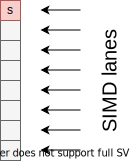
\includegraphics[height=0.5\textheight]{figures/scalarregisteruse.png}
      \end{center}

      Runs at $\frac{1}8$ of possible ADD peak.
    \end{column}
  \end{columns}
\end{frame}

\begin{frame}[fragile]
  \frametitle{Applicable peak (SIMD execution)}
  \begin{columns}
    \begin{column}{0.6\textwidth}\small
      \structure{Scalar code}

\begin{minted}{c}
float c = 0;
for (i = 0; i < N; i++)
  c += a[i];
\end{minted}

      \structure{Assembly pseudo-code}

\begin{minted}[fontsize=\scriptsize, mathescape=true,escapeinside=||]{c}
LOAD [r1.0, ..., r1.7] |$\gets$| [0, ..., 0]
i |$\gets$| 0
loop:
  LOAD [r2.0, ..., r2.7] |$\gets$| [a[i], ..., a[i+7]]
  ADD  r1 |$\gets$| r1 + r2 // SIMD ADD
  i |$\gets$| i + 8
  if i < N: loop
result |$\gets$| r1.0 + r1.1 + ... + r1.7
\end{minted}

    \end{column}
    \begin{column}{0.3\textwidth}
      Using all eight SIMD lanes

      \begin{center}
        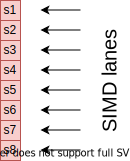
\includegraphics[height=0.5\textheight]{figures/vectorregisteruse.png}
      \end{center}

      Runs at ADD peak.
    \end{column}
  \end{columns}
\end{frame}

\begin{frame}
  \frametitle{Exercise 1: benchmarking sum reduction}
  \begin{enumerate}[itemsep=8pt]
    \item Split into small groups
    \item Make sure one person per group has access to Hamilton
    \item Benchmark sum reduction to confirm this ``theoretical'' effect.
    \item Ask questions!
  \end{enumerate}
\end{frame}

\begin{frame}
  \frametitle{Exercise 1: results}
  \begin{columns}[c]
    \begin{column}{0.27\textwidth}
      \small
      \vskip -50pt
      \begin{itemize}[itemsep=5pt,wide=0pt]
      \item SIMD: 4 plateaus
      \item scalar: 3 plateaus
      \end{itemize}
    \end{column}
    \begin{column}{0.7\textwidth}
      \begin{center}
        \vskip -10pt
        \begin{tikzpicture}
          \begin{axis}[
            height=7cm,
            width=10cm,
            xlabel={Array size},
            ylabel near ticks,
            ylabel={MFlops/s},
            xmode=log,
            xtick={1,16,256,4096,65536,1048576},
            xticklabels={1kB,16kB,256kB,4MB,64MB,1GB},
            log basis x={10},
            style={font=\small},
            legend pos={north east},
            thick,
            legend style={
              cells={anchor=west, align=left},
              fill=bgcolor, font=\footnotesize}
            ]
            \pgfplotstableread[row sep=\\]{%
              kB scalar avx\\
              1 4735.04 25689.32\\
              2 4580.04 35475.57\\
              4 4504.35 40751.21\\
              8 4468.90 37854.32\\
              16 4453.18 36623.58\\
              32 4435.81 34807.33\\
              64 4304.03 25788.06\\
              128 4428.43 26194.16\\
              256 4230.27 26289.56\\
              512 4413.59 22032.32\\
              1024 4363.30 18911.31\\
              2048 4387.13 18827.32\\
              4096 4329.91 18927.51\\
              8192 4354.66 19049.54\\
              16384 4022.46 14018.35\\
              32768 3421.64 5652.13\\
              65536 3430.28 5663.15\\
              131072 3413.95 5671.12\\
              262144 3423.07 5680.15\\
              524288 3422.18 5616.93\\
              1048576 3431.70 5676.13\\
            }\mydata

            \addplot [PineGreen, very thick, mark=asterisk, mark size=2.5pt]
            table[x=kB,y=scalar] {\mydata};
            \addlegendentry{\texttt{sp\_sum}}

            \addplot [Black, very thick, mark=o, mark size=2.5pt]
            table[x=kB, y=avx] {\mydata};
            \addlegendentry{\texttt{sp\_sum\_avx}}

            \addplot[Red, draw=black, dashed, mark=none, very thick] coordinates
            {(1,4735.04)(1048576,4735.04)};
            \addlegendentry {Scalar peak}

            \addplot[Blue, draw=black, mark=none, very thick] coordinates
            {(1,40751.21)(1048576,40751.21)};
            \addlegendentry {SIMD peak}

          \end{axis}
        \end{tikzpicture}
      \end{center}
    \end{column}
  \end{columns}
\end{frame}

\begin{frame}
  \frametitle{Conclusions}
  \begin{itemize}[itemsep=11pt]
  \item Modern computer hardware is quite complex
  \item For simple things we can try to figure our performance limits
  \item Typically we must benchmark to confirm hypotheses
  \item We must find bottlenecks before starting to optimise
  \end{itemize}

  \vskip 20pt

  \structure{Next:} memory hierarchy and first models of performance.
\end{frame}

\end{document}
